\chapter{Marco Teórico}

\section{Fundamentos de la descarga electrostática}

El estudio de la electrostática se remonta a los primeros registros históricos sobre
fenómenos eléctricos. Se atribuye a Tales de Mileto la observación de que, al frotar
un trozo de ámbar con pelo animal o lana, pequeñas partículas de polvo y hojas eran
atraídas hacia el material \cite{ESDA1}. De hecho, la palabra ``electro'' proviene del
griego \textit{elektron}, que significa ámbar.

\begin{figure}[H]
    \centering
    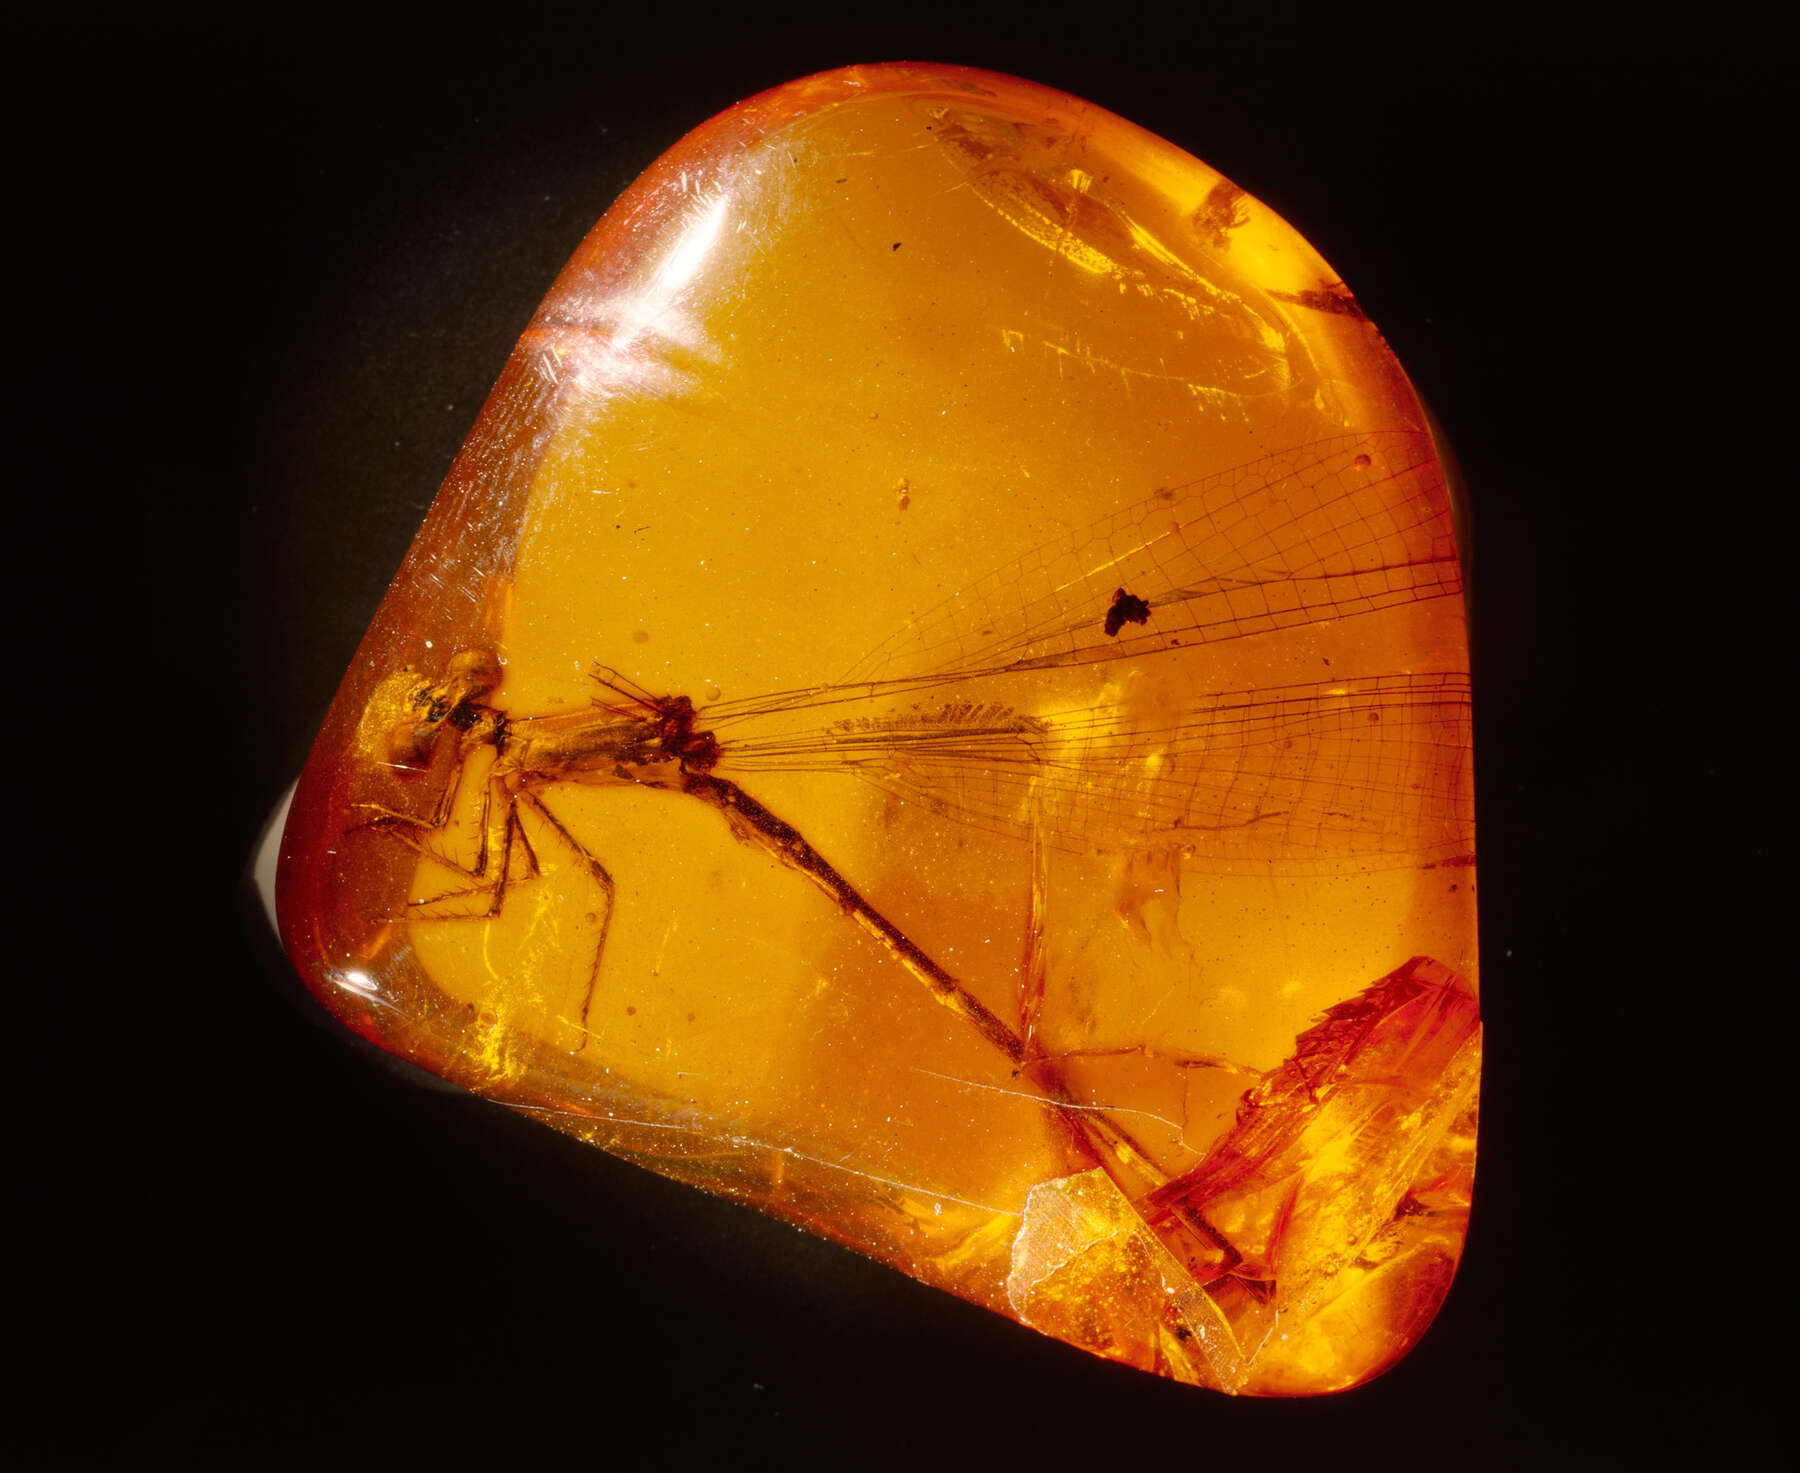
\includegraphics[width=0.4\textwidth]{pics/TF1_1.jpg}
    \caption{Fotografía de un ámbar \cite{Getty_Electrostatics}.}
    \label{fig:ambar_electrostatica}
\end{figure}

En ambientes secos es común que las personas experimenten descargas electrostáticas
al tocar superficies metálicas, por ejemplo después de caminar sobre un piso
alfombrado. Aunque este fenómeno puede parecer inofensivo en situaciones cotidianas,
en la industria electrónica representa un riesgo importante, ya que puede dañar
dispositivos electrónicos o degradar su vida útil. Desde siglos anteriores se han
implementado medidas preventivas frente a la electrostática; por ejemplo, en fuertes
militares europeos y del Caribe se utilizaban prácticas de control electrostático para
reducir el riesgo de ignición en depósitos de pólvora \cite{ESDA1}.

\vspace{2mm}

En la era de la electrónica, la electrostática adquiere una relevancia aún mayor debido
a la reducción continua del tamaño de los circuitos integrados y al incremento de sus
velocidades de operación. Estas características hacen que los dispositivos modernos
sean más sensibles a descargas electrostáticas, por lo que las acciones de control ESD
se han vuelto prioritarias en ambientes donde se manipulan componentes electrónicos
\cite{ESDA1,TI2014}.
En la industria de semiconductores, la electrostática puede afectar el rendimiento de
producción, conocido en inglés como \textit{yield}, así como la calidad y confiabilidad
del producto final \cite{ESDA1,TI2014}. Ignorar este fenómeno puede provocar que dispositivos
electrónicos resulten defectuosos o dañados durante etapas de ensamblaje,
manipulación o prueba \cite{TI2014}.

\subsection{Concepto de ESD}

La electrostática se define como la presencia de cargas eléctricas en reposo. De forma
general, puede entenderse como un desbalance de cargas eléctricas en la superficie de
un material o cuerpo. Este desbalance produce un campo eléctrico que puede medirse y
afectar otros objetos cercanos. En este sentido, las cargas electrostáticas pueden
asociarse con energía potencial almacenada. Una característica importante de la
descarga electrostática es su corta duración, ya que puede ocurrir en el orden de
picosegundos o nanosegundos. Además, el campo eléctrico generado puede alcanzar
valores elevados \cite{ESDA1}, lo que permite observar fenómenos como el mostrado en
la Figura~\ref{fig:experimento_electrostatica}.

\begin{figure}[H]
    \centering
    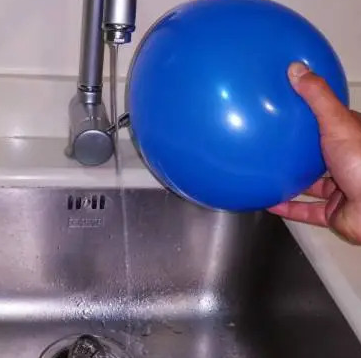
\includegraphics[width=0.4\textwidth]{pics/TF1_2.png}
    \caption{Experimento de electrostática \cite{Globos_Electrostatica}.}
    \label{fig:experimento_electrostatica}
\end{figure}

Usualmente, una descarga electrostática ocurre por medio de una chispa o destello
generado por la diferencia de potencial electrostático entre dos objetos o cuerpos.
Conforme estos se acercan, el campo eléctrico puede superar la rigidez dieléctrica del
aire y producir una descarga, como se ilustra en la Figura~\ref{fig:van_graaff}.

\begin{figure}[H]
    \centering
    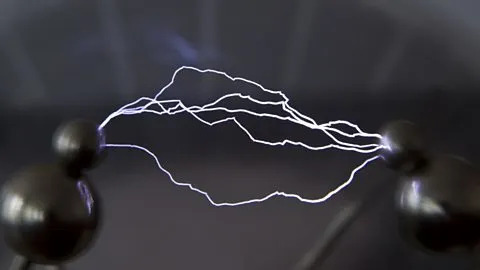
\includegraphics[width=0.5\textwidth]{pics/TF1_3.jpg}
    \caption{Chispa electrostática usando un generador de Van Graaff \cite{BBC_Static}.}
    \label{fig:van_graaff}
\end{figure}

La generación de cargas electrostáticas inicia con el contacto y separación de dos
materiales. Este fenómeno, comúnmente asociado al frotamiento, puede ocurrir entre
materiales similares o diferentes; sin embargo, cuando los materiales son distintos, la
carga generada suele ser mayor. Algunos ejemplos comunes son una persona caminando
sobre un piso alfombrado o un dispositivo electrónico deslizándose dentro o fuera de
una bolsa, revista o paño.

Este mecanismo de generación de carga se conoce como carga triboeléctrica. Cuando dos
materiales eléctricamente neutros entran en contacto y luego se separan, puede ocurrir
una transferencia de carga, de modo que uno de los materiales queda cargado
positivamente y el otro negativamente \cite{ESDA1}. Este proceso se representa en la
Figura~\ref{fig:carga_triboelectrica}.

\begin{figure}[H]
    \centering
    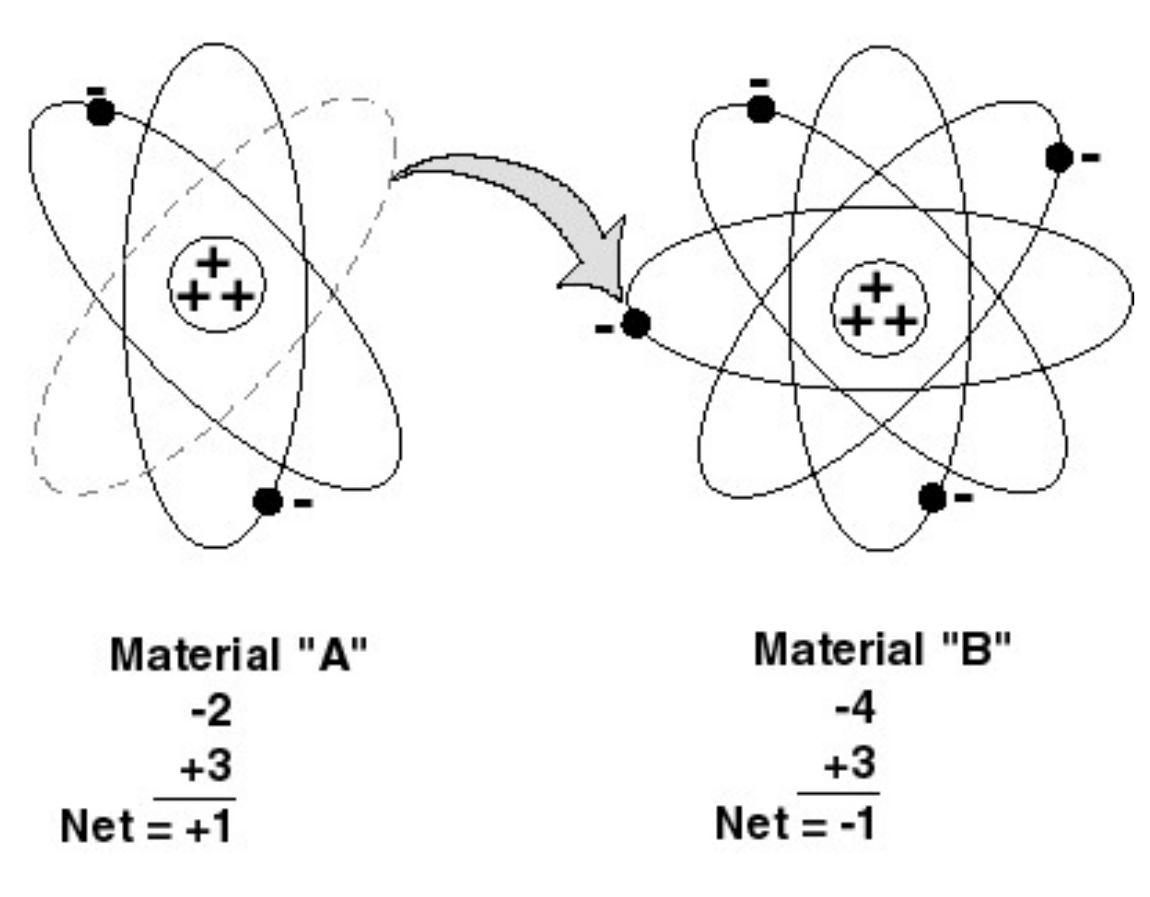
\includegraphics[width=0.55\textwidth]{pics/TF1_4.png}
    \caption{Ilustración de generación de una carga triboeléctrica \cite{ESDA1}.}
    \label{fig:carga_triboelectrica}
\end{figure}

La carga eléctrica se mide en coulombs. En electrostática, una relación comúnmente
utilizada es la ecuación de capacitancia, donde $q$ representa la carga eléctrica, $C$ la
capacitancia del material, objeto o cuerpo, y $V$ el potencial eléctrico:

\begin{equation}
    q = CV
    \label{eq:carga_capacitancia}
\end{equation}

Un coulomb equivale aproximadamente a $6.2415 \cdot 10^{18}$ cargas eléctricas, ya
sean electrones o protones \cite{Illinois_Static}. Sin embargo, en aplicaciones de
control ESD suele ser más común referirse al potencial electrostático, expresado en
voltios, o al campo electrostático, expresado en voltios por metro.

\subsection{Modelo de ESD HBM}

Las descargas electrostáticas pueden ocurrir por diferentes fuentes. Debido a esto, los
estándares definen modelos eléctricos para representar distintos escenarios y establecer
umbrales de sensibilidad que permitan evaluar la integridad de los dispositivos
electrónicos ante una descarga electrostática. Entre los modelos más conocidos se
encuentran el HBM (\textit{Human Body Model}), el CDM (\textit{Charged Device Model})
y el MM (\textit{Machine Model}). Para este proyecto, el análisis se centra
principalmente en el modelo HBM.

\vspace{2mm}

Una de las principales fuentes de daño por ESD corresponde a las descargas generadas
por personas hacia materiales u objetos sensibles. En algunas ocasiones, la carga
acumulada en el cuerpo humano puede alcanzar potenciales suficientemente altos para
producir una ruptura dieléctrica del aire, de modo que la descarga puede ocurrir incluso
sin contacto directo, siempre que exista una distancia suficientemente pequeña entre el
usuario y el dispositivo afectado \cite{esda_part5}. Este caso se representa mediante el
modelo HBM, el cual describe la descarga electrostática desde el cuerpo humano hacia un
dispositivo.

\begin{figure}[H]
    \centering
    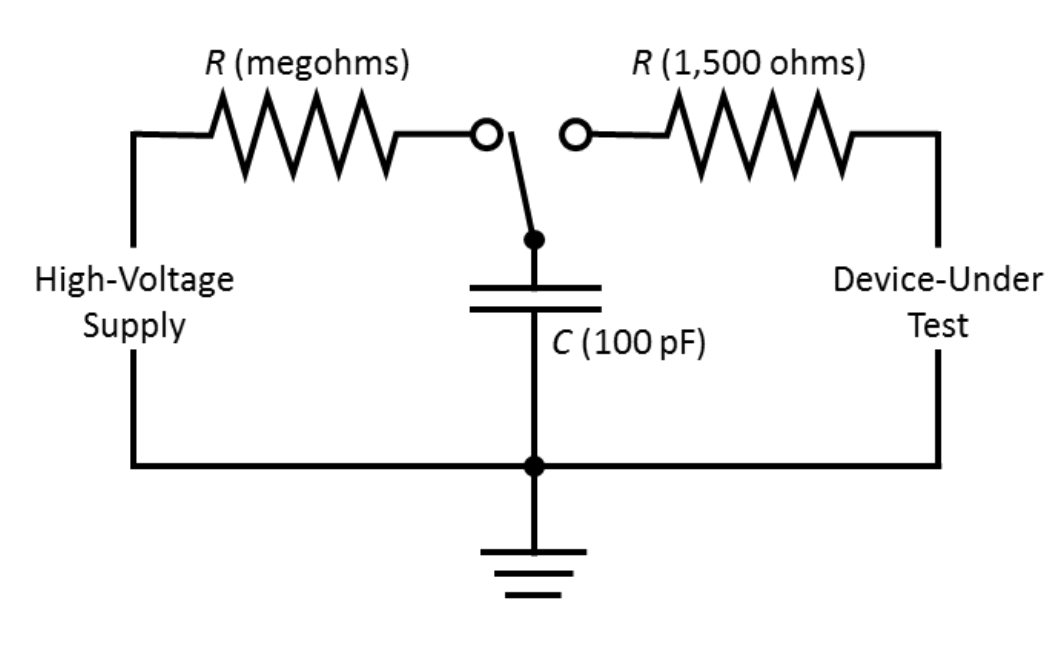
\includegraphics[width=0.55\textwidth]{pics/TF1_5.png}
    \caption{Modelo HBM simplificado \cite{esda_part5}.}
    \label{fig:modelo_hbm}
\end{figure}

En este modelo, mostrado en la Figura~\ref{fig:modelo_hbm}, la fuente de alto voltaje
representa la transferencia de carga electrostática hacia el cuerpo. El cuerpo humano
puede modelarse como una impedancia con componente resistivo y capacitivo, donde la
energía se almacena principalmente debido a su comportamiento capacitivo.
Posteriormente, la trayectoria de descarga hacia el dispositivo incluye una resistencia
asociada al contacto y al camino de descarga.

\vspace{2mm}

La forma de onda de una descarga HBM se caracteriza por un tiempo de levantamiento en
el orden de nanosegundos, una corriente pico dependiente del nivel de tensión aplicado y
una caída doblemente exponencial. En este tipo de evento, la falla del dispositivo se
asocia principalmente con la energía transferida durante el pulso HBM \cite{esda_part5}.
La Figura~\ref{fig:pulso_hbm} muestra un ejemplo representativo de este tipo de pulso.

\begin{figure}[H]
    \centering
    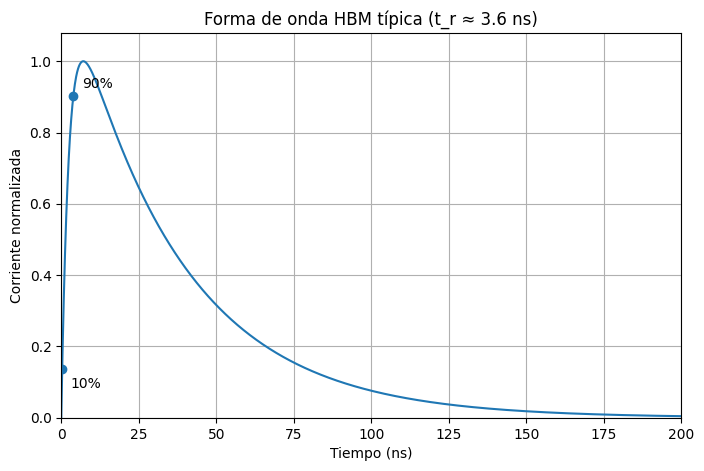
\includegraphics[width=0.65\textwidth]{pics/TF1_6.png}
    \caption{Ejemplo de un pulso HBM. Fuente: elaboración propia.}
    \label{fig:pulso_hbm}
\end{figure}

Los dispositivos electrónicos sensibles a ESD pueden clasificarse según su nivel de
sensibilidad ante el modelo HBM. Distintos estándares, como ANSI/ESDA y JEDEC,
establecen rangos de clasificación como los mostrados en la Tabla~\ref{tab:hbm}.

\begin{table}[H]
\centering
\caption{Clasificación de componentes ESD según el modelo HBM (ANSI/ESDA/JEDEC JS-001).}
\begin{tabular}{|c|c|}
\hline
\textbf{Clasificación} & \textbf{Rango de voltaje (V)} \\
\hline
0Z & $< 50$ \\
0A & $50$ a $< 125$ \\
0B & $125$ a $< 250$ \\
1A & $250$ a $< 500$ \\
1B & $500$ a $< 1000$ \\
1C & $1000$ a $< 2000$ \\
2  & $2000$ a $< 4000$ \\
3A & $4000$ a $< 8000$ \\
3B & $\geq 8000$ \\
\hline
\end{tabular}
\label{tab:hbm}
\end{table}

Los daños físicos producidos por una descarga electrostática pueden observarse a nivel
de estructuras internas del circuito integrado. Texas Instruments muestra ejemplos de
daños en transistores y óxidos de compuerta ocasionados por eventos ESD, como se
presenta en la Figura~\ref{fig:danos_circuitos_esd}.

\begin{figure}[H]
\centering

\begin{subfigure}[t]{0.45\textwidth}
    \centering
    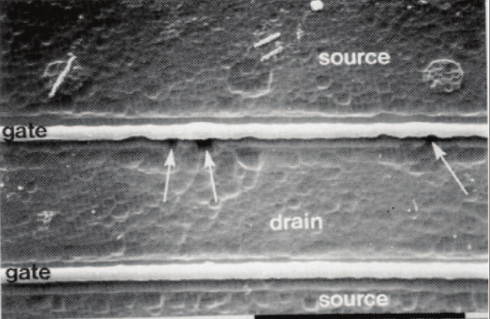
\includegraphics[width=\textwidth]{pics/TF1_7.png}
    \caption{Daño en la unión de drenador y fuente de un transistor NMOS después de
    un estrés HBM \cite{TI2014}.}
    \label{fig:dano_hbm}
\end{subfigure}
\hfill
\begin{subfigure}[t]{0.45\textwidth}
    \centering
    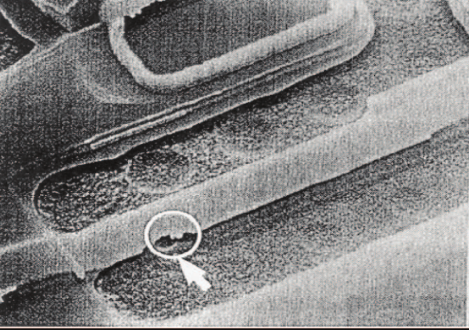
\includegraphics[width=\textwidth]{pics/TF1_8.png}
    \caption{Daño en el óxido de compuerta de un buffer después de un estrés CDM
    \cite{TI2014}.}
    \label{fig:dano_cdm}
\end{subfigure}

\caption{Daños en circuitos integrados debido a ESD.}
\label{fig:danos_circuitos_esd}
\end{figure}

\subsection{Influencia del ambiente}

Una de las principales variables que influyen en la generación de carga electrostática es
la humedad relativa del ambiente. Cuando la humedad relativa disminuye, se reduce la
capacidad del entorno para disipar carga, lo que favorece la acumulación de potencial
electrostático en materiales y personas \cite{versalogic_esd}. La Tabla~\ref{tab:esd_humidity}
muestra ejemplos de potenciales típicos generados bajo diferentes condiciones de humedad
relativa.

\begin{table}[H]
    \centering
    \caption{Potenciales típicos generados en una persona según la HR y el medio.}
    \begin{tabularx}{\linewidth}{Xcc}
    \toprule
    \textbf{Medio de generación} & \textbf{10--25\% HR} & \textbf{65--90\% HR} \\
    \midrule
    Caminar sobre alfombra & 35,000 V & 15,000 V \\
    Caminar sobre baldosa de vinilo & 12,000 V & 250 V \\
    Trabajar en banco & 6,000 V & 100 V \\
    Bolsa plástica levantada del banco & 20,000 V & 1,200 V \\
    Sentado en silla con espuma de uretano & 18,000 V & 1,500 V \\
    \bottomrule
    \end{tabularx}
    \label{tab:esd_humidity}

    {\small Fuente: basado en \cite{versalogic_esd}.}
\end{table}

Una explicación de este comportamiento es que la humedad relativa está asociada con la
presencia de moléculas de agua en el aire. Estas moléculas pueden facilitar la disipación
de carga electrostática hacia tierra, reduciendo la acumulación de potencial en el cuerpo
o en los materiales. Cuando la humedad relativa es baja, el cuerpo puede quedar más
aislado del plano de tierra y adquirir mayores niveles de carga electrostática. Por esta
razón, los sistemas de control ESD verifican la resistencia del usuario hacia tierra, ya
que mantener este valor dentro de un rango aceptable permite favorecer una disipación
controlada de carga y reducir el riesgo para dispositivos electrónicos sensibles
\cite{versalogic_esd}.

\section{Medición de resistencia cuerpo a tierra}

Uno de los conceptos fundamentales para este proyecto es la medición de resistencia del
cuerpo a tierra, conocida en inglés como \textit{body-to-ground resistance}. En un
laboratorio, el plano de referencia a tierra suele estar asociado con el sistema de puesta a
tierra del área de trabajo o con superficies disipativas conectadas a tierra. El objetivo es
que el usuario presente una resistencia eléctrica hacia tierra dentro de un rango específico,
usualmente en el orden de los M$\Omega$ \cite{STM97_ANSI}. La
Figura~\ref{fig:medicion_resistencia_cuerpo_tierra} ilustra este principio de medición.

\begin{figure}[H]
    \centering
    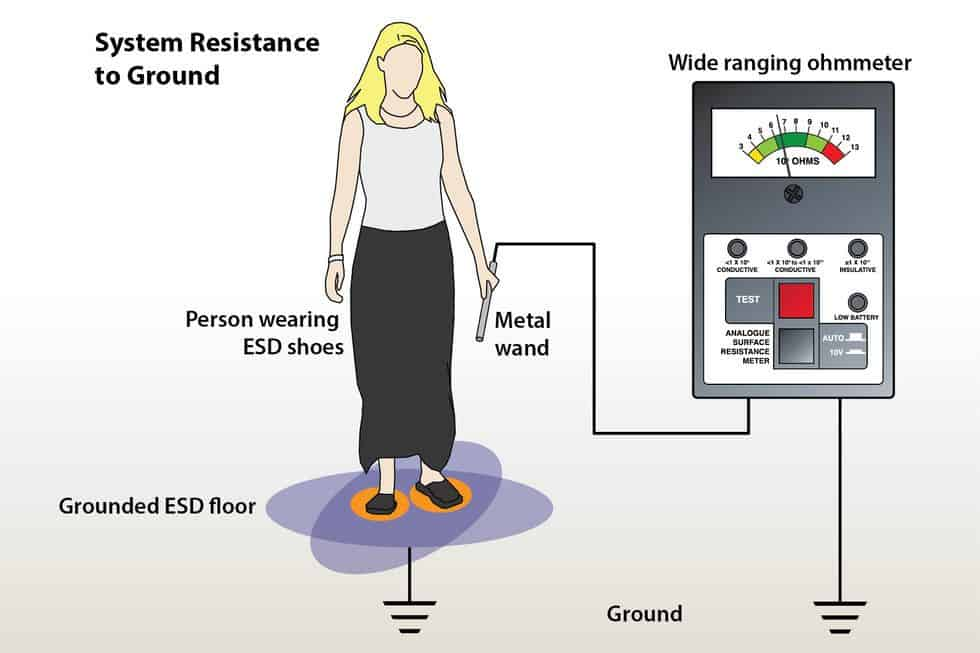
\includegraphics[width=0.65\textwidth]{pics/TF2_1.jpg}
    \caption{Ilustración de medición de resistencia de cuerpo a tierra \cite{STM97_ANSI}.}
    \label{fig:medicion_resistencia_cuerpo_tierra}
\end{figure}

Esta medición debe realizarse mediante estímulos eléctricos en DC, de acuerdo con los
métodos establecidos en las normas aplicables. Un aspecto importante es que el cuerpo
humano puede modelarse como una impedancia dependiente de diferentes variables:

\begin{equation}
    Z_{Cuerpo} = R\text{(f,V,P,A,H)} + jX\text{(f,V,P,A,H)}
    \label{eq:impedancia_cuerpo}
\end{equation}

La resistencia eléctrica del cuerpo humano no es constante ni lineal, sino que depende de
factores como la frecuencia, la presión de contacto, el área de
contacto y la humedad de la piel del usuario\cite{khalil2014bioimpedance}, 
también factores como la tensión de estímulo,  
la humedad relativa del ambiente pueden afectarla . La reactancia también depende
de estas variables, aunque generalmente su variación es menos significativa que la del
componente resistivo \cite{ELEK_IEC_IEEE_Safety_2023}. El componente reactivo del
cuerpo tiene un comportamiento principalmente capacitivo, lo cual se relaciona con la
capacidad del cuerpo para almacenar energía electrostática, como se observa en el modelo
HBM \cite{dtic_skin}. Para fines de este proyecto, el análisis se centra en la medición en
DC, por lo que se considera $f=0$ Hz como condición de medición.

Debido a que los estándares establecen la medición de la resistencia del usuario mediante
una señal DC \cite{S1_1_ANSI}, la frecuencia deja de considerarse como variable de
operación. Las tensiones de prueba dependen del tipo de dispositivo; por ejemplo, algunos
equipos portátiles aplican señales del orden de 4 V \cite{Desco_19240}, mientras que en
equipos no portátiles es común encontrar valores cercanos a 30 V \cite{Desco_SmartLog}.

\begin{figure}[H]
    \centering
    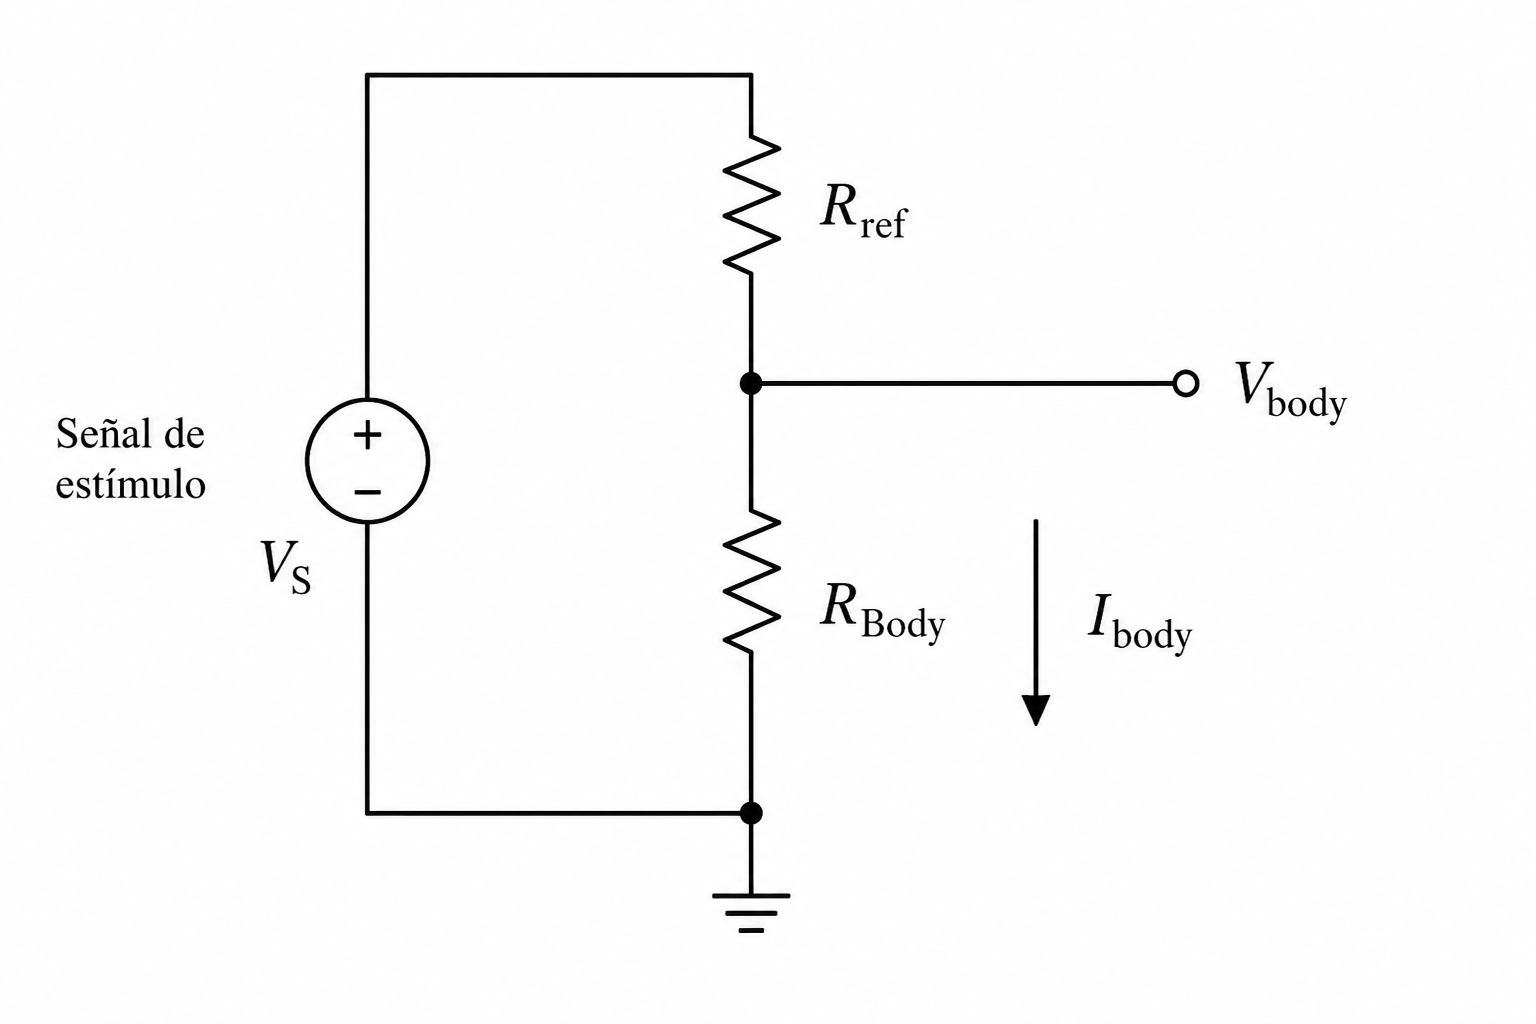
\includegraphics[width=0.65\textwidth]{pics/TF3_4.png}
    \caption{Uso de divisor de tensión para medición de la resistencia del cuerpo a
    tierra. Fuente: elaboración propia.}
    \label{fig:divisor_resistencia_tierra}
\end{figure}

Las estaciones de control ESD utilizan como base la ley de Ohm para obtener
el valor de resistencia del cuerpo a tierra. Un divisor de tensión, como el mostrado en la
Figura~\ref{fig:divisor_resistencia_tierra}, es una estrategia común en este tipo de
mediciones, ya que a partir del valor medido de $V_{body}$ y de los valores conocidos de
$R_{ref}$ y $V_s$, es posible estimar $R_{Body}$ \cite{keithley_lowlevel}.

Un aspecto importante es que la medición de la resistencia de una persona requiere de conectar
electricamente a el usuario al circuito electrónico de medición, similar a la medición de una señal 
de electrocardiograma por ejemplo donde se colocan electrodos al usuario para conectar electricamente al usuario 
al sistema electrónico de la misma forma los dispositivos de medición de resistencia eléctrica para 
personas requieren que el usuario realize contacto con alguna superficie metálica destinada para cerrar 
el circuito y asi poder realizar la medición \cite{STM97_ANSI}. 

\begin{figure}[H]
    \centering
    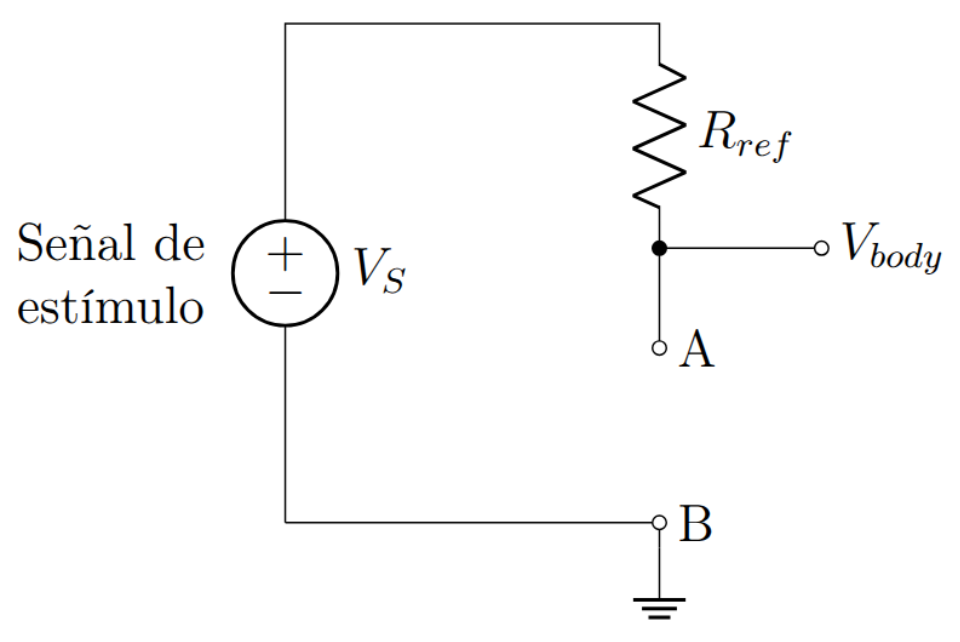
\includegraphics[width=0.65\textwidth]{pics/TF9.png}
    \caption{Ejemplo de puntos de conexión para medición de resistencia del cuerpo a tierra. Fuente: elaboración propia.}
    \label{fig:ilustracion_resistencia_tierra}
\end{figure}

Es usual en los circuitos electrónicos para estos fines que la terminal A se conecte a la punta del dedo índice del usuario y la 
terminal B puede variar entre si se desea probar una pulsera antiestática para muñeca o tobillo, donde en caso que sea para muñeca la 
terminal B correspondería a la terminal tipo banana de la pulsera, esto debido a que se espera que la pulsera se conecte en una estación de 
trabajo que estará conectada a la tierra eléctrica del edificio. En caso de pulseras antiestática para tobillo se utiliza un plato metálico 
donde el usuario debe colocar ambos pies y entonces la terminal B se va a alternar entre el pie derecho o izquierdo para medir ambas resistencias y 
evaluar que esten dentro del rango de Ohms definido por los estándares \cite{smartlogpro2_manual}.

\begin{figure}[H]
    \centering
    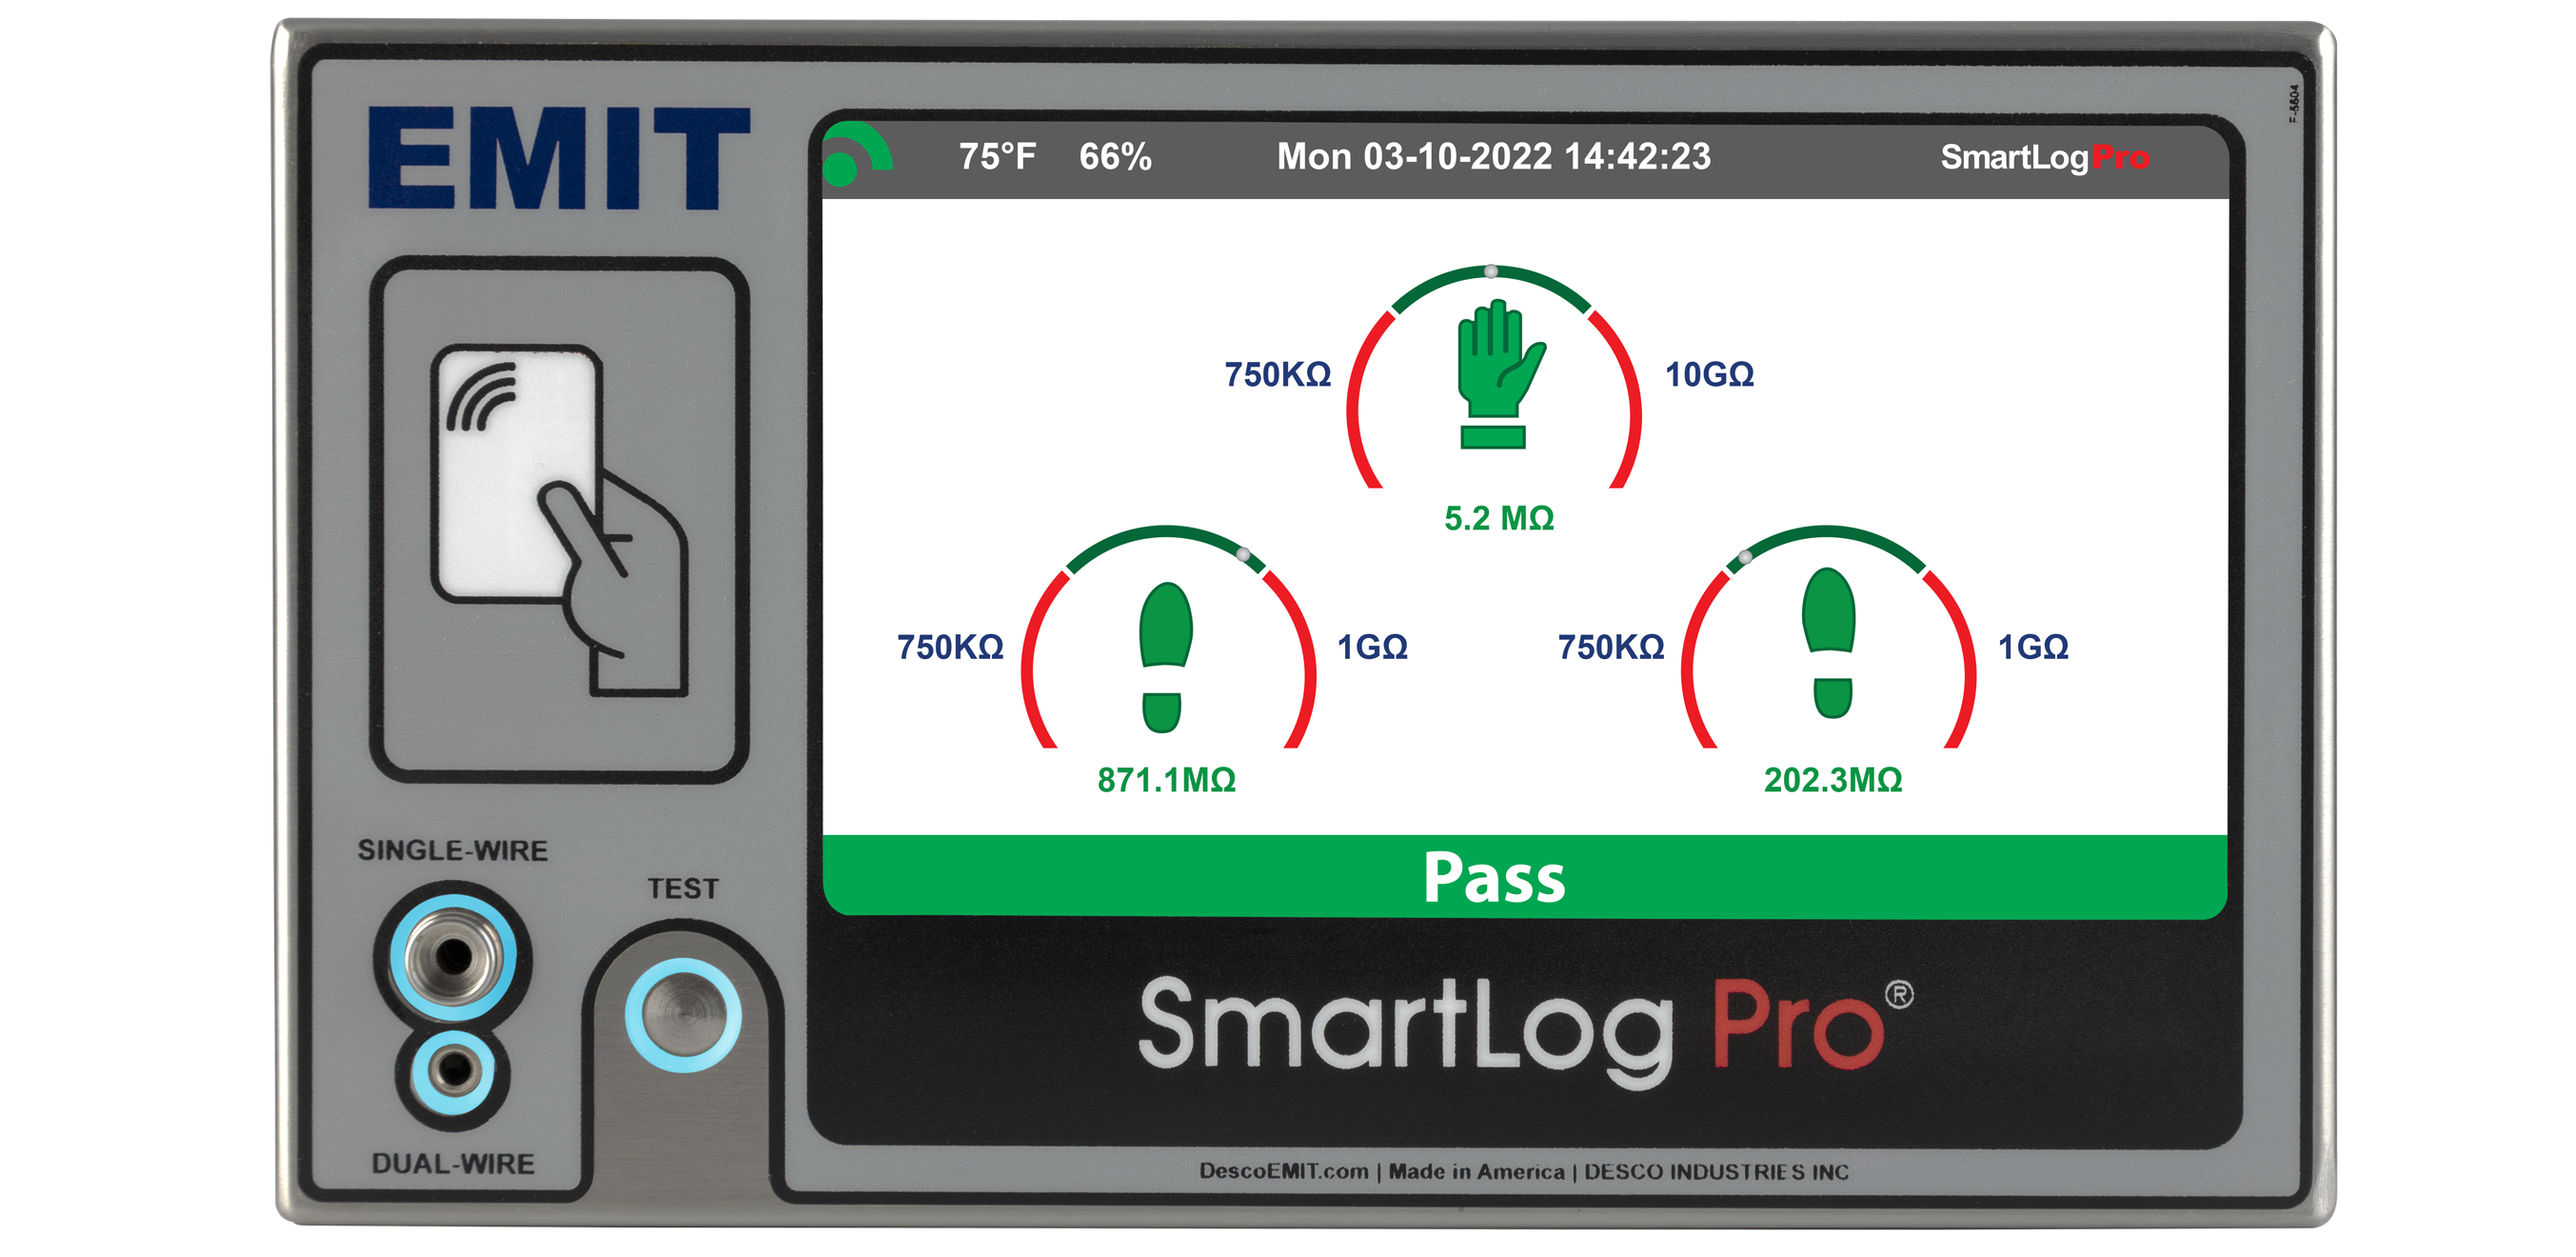
\includegraphics[width=0.65\textwidth]{pics/TF10.png}
    \caption{Puntos de medición de la estación de ESD SmartLog Pro 2. Fuente: \cite{SmartLogPro2}.}
    \label{fig:puntos_medicion_smartlog_pro2}
\end{figure}

Sin embargo esto representa que se deban considerar medidas de seguridad para garantizar que el usuario no tendrá ninguna electrocusión, 
una variable que debe permanecer controlada es la corriente eléctrica que pasará por el usuario cuando se cierre el circuito, estándares 
como el IEC 60601-1 definen normas de seguridad a seguir en estos casos \cite{iec60601_1}, criterios como el uso de corrientes 
menores a los 10 $\mu A$ por ejemplo, se definen en estas normas. Esto es importate de destacar ya que los circuitos electrónicos utilizados
para la medición de la resistencia del cuerpo a tierra de una persona en controles ESD deben asegurar que la corriente eléctrica que pasará 
por el usuario durante la prueba se mantenga dentro de los margenes seguros \cite{S1_1_ANSI}.

\section{Medición de alta impedancia}

La medición de la resistencia cuerpo-tierra se realiza en rangos de alta impedancia. En
estas condiciones, las corrientes involucradas pueden encontrarse en el orden de $\mu$A
o nA, por lo que las corrientes de fuga, el ruido eléctrico y la interferencia
electromagnética pueden introducir errores significativos. Por esta razón, los equipos
utilizados para este tipo de medición deben considerar criterios de aislamiento, precisión
y control de errores \cite{keithley_lowlevel}.

\subsection{Corrientes de fuga}

Las corrientes de fuga representan una fuente importante de error en la medición de altas
impedancias. Aunque estas corrientes pueden encontrarse en el orden de $\mu$A o nA, su
valor puede ser comparable con la corriente que circula a través del elemento bajo prueba.
Como resultado, la corriente medida incluye tanto la corriente de interés como las
contribuciones parásitas presentes en los cables, los materiales aislantes y la tarjeta
electrónica. Para disminuir este efecto se deben utilizar materiales con buen aislamiento,
reducir la contaminación superficial y considerar la influencia de la humedad
\cite{keithley_lowlevel}.

\subsection{Efectos de EMI y ruido}

Las pequeñas corrientes presentes en una medición de alta impedancia hacen que el sistema
sea sensible al ruido eléctrico y a la interferencia electromagnética. Estas perturbaciones
pueden acoplarse mediante el cuerpo del usuario, los cables o las pistas de la tarjeta
electrónica y producir variaciones en el resultado. El uso de cables blindados, una
distribución adecuada de las conexiones y la reducción del ancho de banda mediante
filtrado permiten disminuir estos efectos \cite{keithley_lowlevel}.

\subsection{Técnicas de guardado (guarding)}

El guardado es una técnica utilizada para reducir las corrientes de fuga en trayectorias de
alta impedancia. Consiste en mantener las regiones cercanas a la señal sensible a un
potencial similar, de forma que la diferencia de tensión entre ellas sea pequeña. Al
reducirse esta diferencia de potencial, también disminuye la corriente parásita que puede
alterar la medición. Esta técnica puede aplicarse mediante conductores de guarda en la
tarjeta electrónica o mediante cables triaxiales \cite{keithley_lowlevel}.

\subsection{Circuitos para medición de altas impedancias}

La medición de altas impedancias puede realizarse mediante electrómetros,
picoamperímetros o circuitos basados en amplificadores operacionales con corrientes de
polarización bajas. Una alternativa consiste en aplicar una tensión conocida y medir la
corriente resultante, mientras que otra consiste en aplicar una corriente conocida y medir
la tensión producida en el elemento bajo prueba. En ambos casos, el circuito requiere
componentes de precisión, una impedancia de entrada elevada y un diseño que permita
reducir las corrientes de fuga y el ruido antes de adquirir la señal mediante un convertidor
analógico-digital \cite{keithley_lowlevel}.

\section{Protocolo de comunicación ESP-NOW}

ESP-NOW es un protocolo de comunicación inalámbrica desarrollado por Espressif
Systems para el intercambio directo de datos entre dispositivos de la familia
ESP. A diferencia de una conexión Wi-Fi convencional, no requiere que los
dispositivos se asocien con un punto de acceso, obtengan una dirección IP o
utilicen protocolos de transporte como TCP o UDP. Esta característica permite
establecer enlaces locales con poca infraestructura y una menor sobrecarga de
comunicación, lo cual resulta útil en sistemas embebidos e Internet de las
Cosas (IoT) \cite{ESPNOWGUIDE,ESPNOWDOC}.

Para ubicar conceptualmente el protocolo puede utilizarse el modelo de
interconexión de sistemas abiertos (OSI), el cual organiza las funciones de
comunicación en las siete capas mostradas en la
Figura~\ref{fig:modelo_osi_siete_capas} \cite[p.~28]{OSIModel}.

\begin{figure}[H]
    \centering
    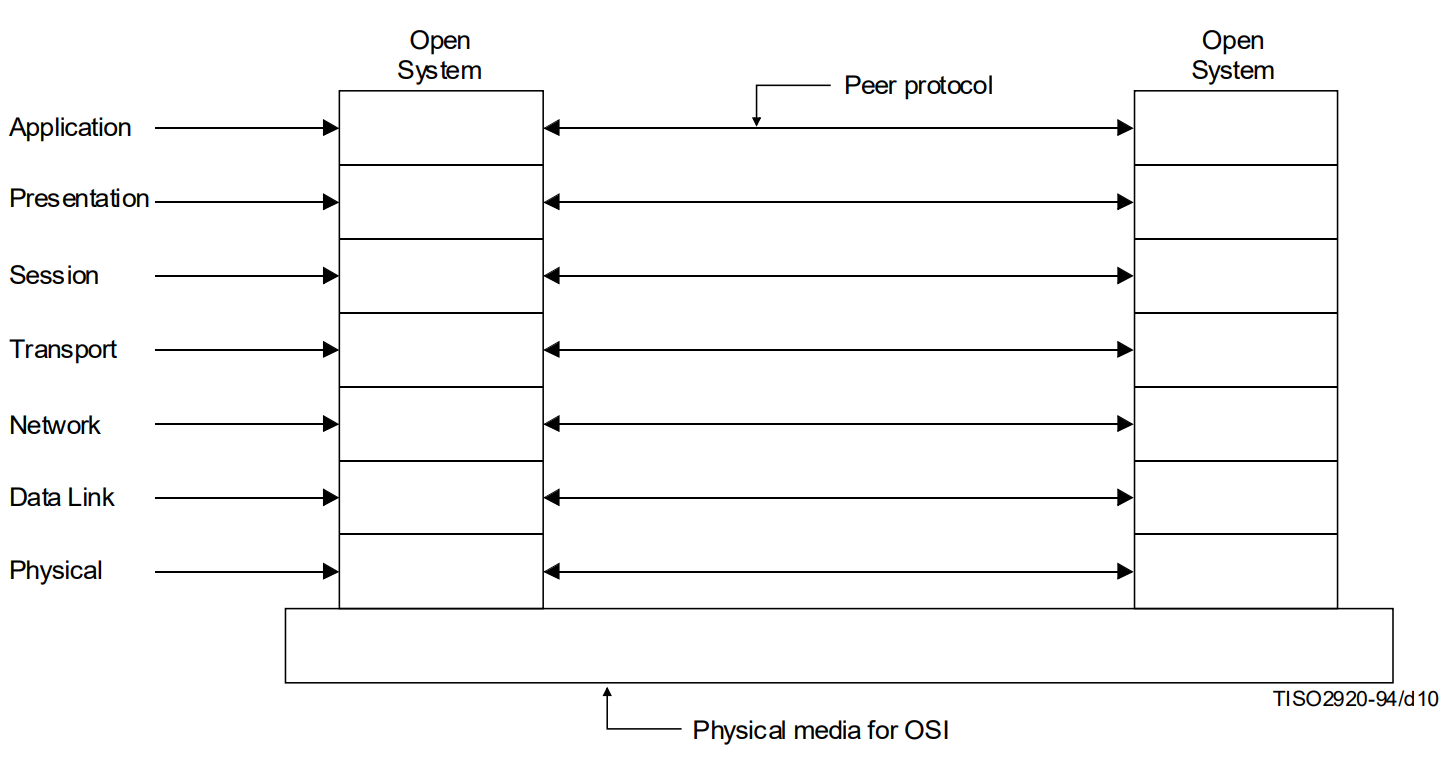
\includegraphics[width=\textwidth]{pics/TF_01.png}
    \caption{Modelo de referencia OSI de siete capas y protocolos entre pares
    \cite[p.~28]{OSIModel}.}
    \label{fig:modelo_osi_siete_capas}
\end{figure}

Tanto ESP-NOW como Wi-Fi convencional emplean la interfaz de radio IEEE 802.11
del microcontrolador. Esta tecnología proporciona funciones asociadas
principalmente con las capas física y de enlace de datos. En ESP-NOW, la
información se transporta mediante tramas de acción específicas del fabricante
y se identifican los dispositivos por sus direcciones MAC
\cite{ESPNOWDOC}. Por tanto, ESP-NOW no elimina las funciones de IEEE 802.11;
su principal simplificación consiste en permitir el intercambio de mensajes sin
la infraestructura y los protocolos de capas superiores utilizados normalmente
en una red Wi-Fi.

\begin{figure}[H]
    \centering
    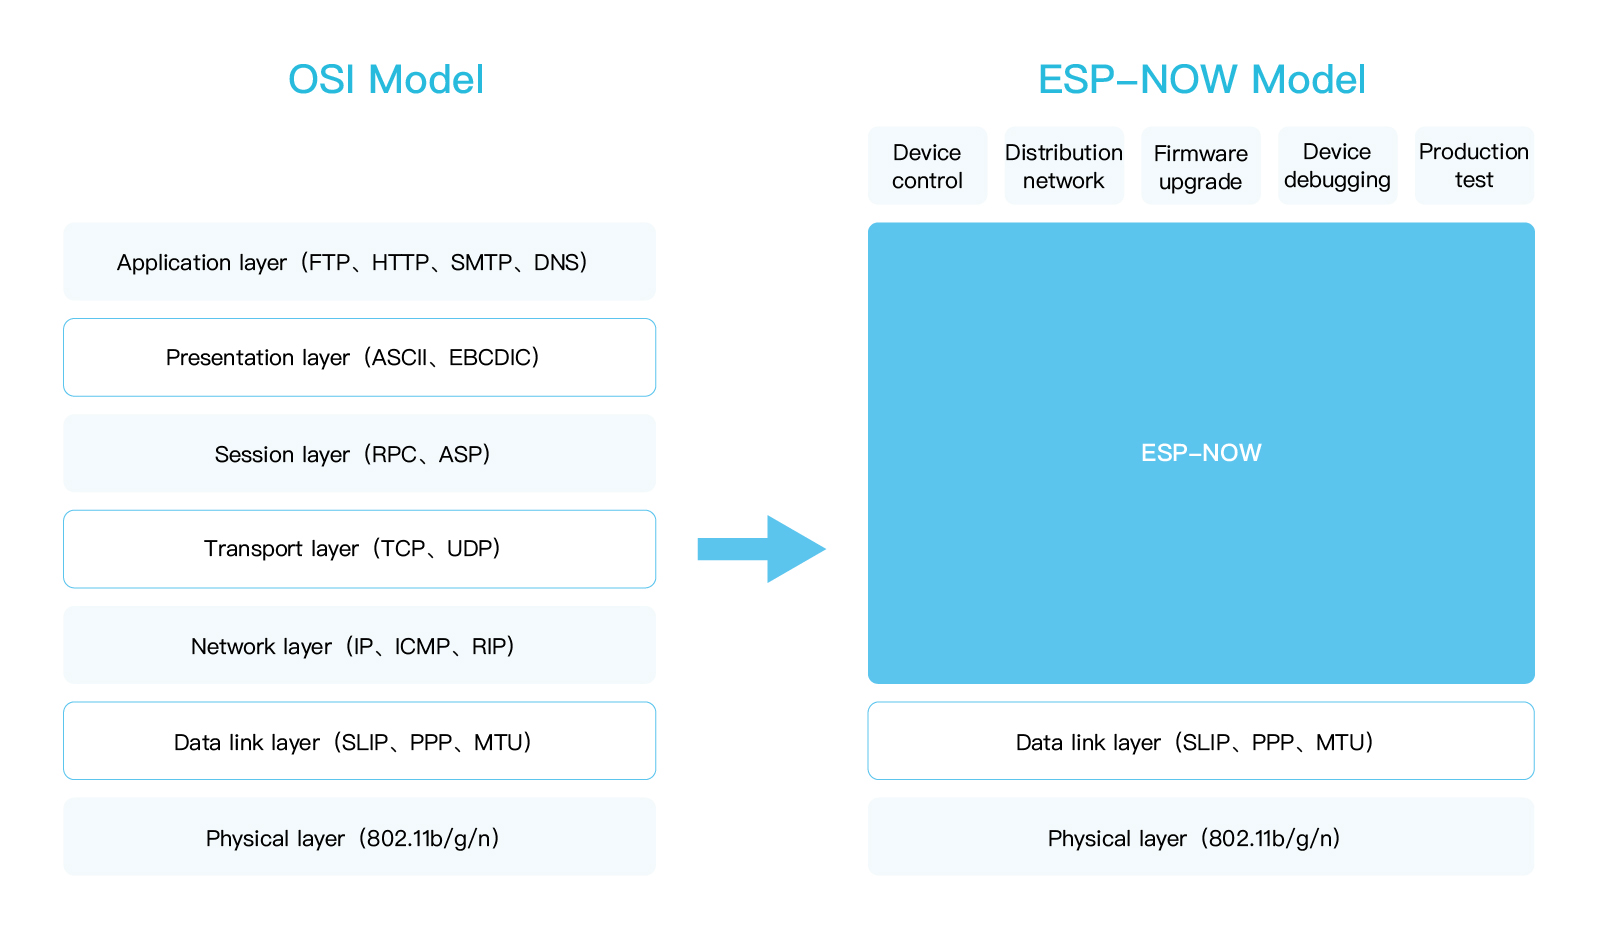
\includegraphics[width=\textwidth]{pics/TF_02.png}
    \caption{Simplificación de la comunicación mediante ESP-NOW en comparación con Wi-Fi
    convencional \cite{ESPNOWGUIDE}.}
    \label{fig:flujo_reconocimiento_espwho}
\end{figure}


La documentación de Espressif denomina iniciador al dispositivo que comienza
un intercambio y respondedor al que recibe la solicitud. Estos roles no son
permanentes: un mismo dispositivo puede enviar y recibir mensajes según la
operación realizada, como se ilustra en la
Figura~\ref{fig:roles_espnow} \cite{ESPNOWGUIDE}.

\begin{figure}[H]
    \centering
    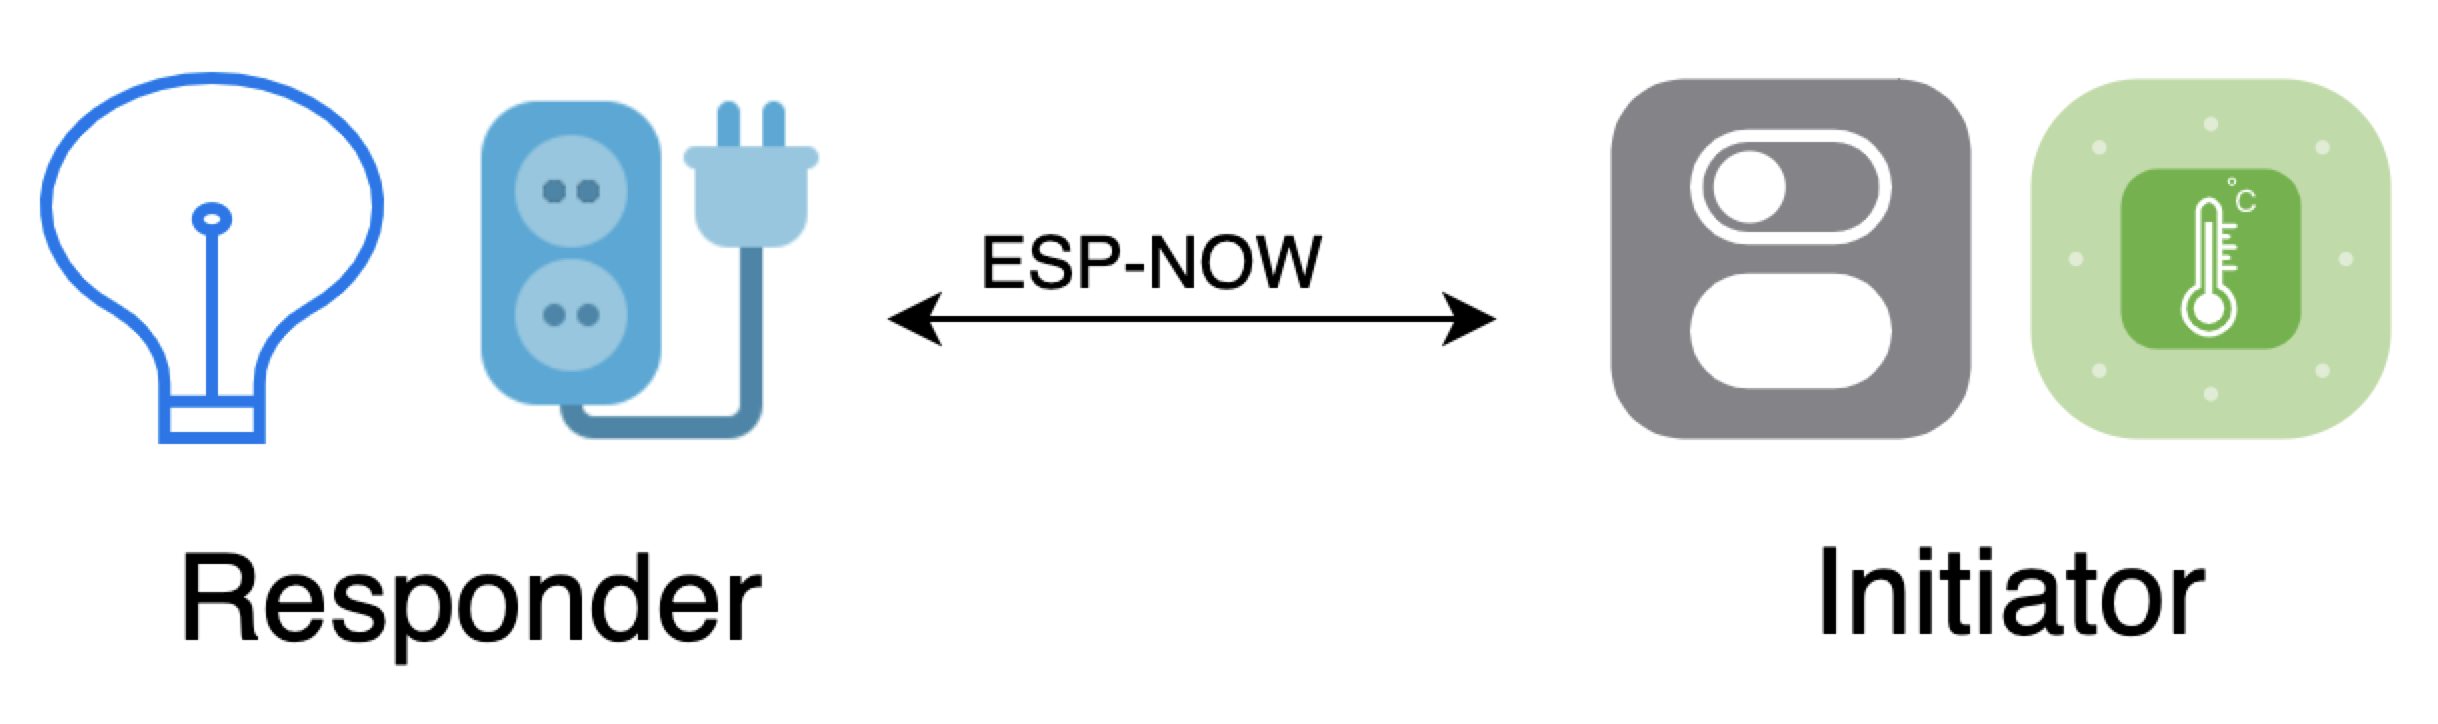
\includegraphics[width=\textwidth]{pics/TF_03.png}
    \caption{Ejemplo de comunicación directa entre un iniciador y un
    respondedor mediante ESP-NOW \cite{ESPNOWGUIDE}.}
    \label{fig:roles_espnow}
\end{figure}

Las características de mayor relevancia para el sistema propuesto se resumen a
continuación \cite{ArduinoESPNOW,ESPNOWDOC}:

\begin{itemize}
    \item Comunicación directa en la banda de 2,4 GHz sin requerir un punto de
    acceso o router.
    \item Operación uno a uno, uno a varios o varios a varios, con un máximo de
    20 dispositivos pares registrados.
    \item Carga útil máxima de 250 bytes en ESP-NOW versión 1.0 y de 1470 bytes
    en la versión 2.0.
    \item Dependencia del canal de radio seleccionado y susceptibilidad a
    interferencias de otros equipos que operen en la misma banda.
\end{itemize}

ESP-NOW organiza la información en tramas, es decir, bloques de datos que
contienen el mensaje y la información necesaria para enviarlo. El protocolo
permite detectar errores durante la transmisión y notifica al emisor si la
trama fue entregada en la capa MAC. Sin embargo, esta notificación no garantiza
que el programa del dispositivo receptor haya procesado el mensaje. Cuando se
requiere mayor confiabilidad, el receptor puede enviar una confirmación y el
emisor puede utilizar números de secuencia o volver a transmitir el mensaje si
no recibe una respuesta \cite{ESPNOWDOC}. La tasa física predeterminada es de
1 Mbps, aunque el rendimiento efectivo depende de la distancia, el canal y las
condiciones de interferencia.

ESP-NOW también puede utilizarse para enviar una actualización de firmware sin
conectar físicamente el dispositivo. Para realizar este proceso, la aplicación
debe dividir el archivo en partes, verificar los datos recibidos y escribir la
nueva versión en la memoria del dispositivo \cite{ESPNOWGUIDE}. En el sistema
propuesto, su función principal es el envío de
mensajes cortos de estado, mediciones y comandos entre los microcontroladores.
La comunicación directa permite que estos intercambios no dependan de la
disponibilidad de un router externo y mantiene una arquitectura local adecuada
para la estación de verificación ESD.

\section{Algoritmos ligeros de visión artificial}

La visión artificial permite que un sistema obtenga información a partir de
imágenes. Entre sus aplicaciones se encuentran la detección de personas, el
reconocimiento facial y la identificación de objetos. En una computadora de
alto desempeño estas tareas pueden ejecutarse con modelos grandes; sin embargo,
un sistema embebido dispone de menos memoria y capacidad de procesamiento. Por
esta razón, la selección del algoritmo debe considerar no solo su exactitud,
sino también el espacio de almacenamiento, la memoria de trabajo, el tiempo de
respuesta y el consumo de energía \cite{TinyMLReview2022,MCUNet2020}.

El aprendizaje automático (\textit{Machine Learning}, ML) permite que un sistema
encuentre patrones a partir de datos. Cuando se ejecuta en microcontroladores
con recursos limitados suele denominarse TinyML (\textit{Tiny Machine
Learning}). Su propósito es resolver localmente una tarea concreta con memoria,
costo y consumo reducidos, no sustituir una computadora de alto desempeño. El
procesamiento local también disminuye la dependencia de servicios externos y
evita transmitir continuamente las imágenes capturadas
\cite{TinyMLReview2022}.

\subsection{Funcionamiento básico del reconocimiento facial}

La detección facial localiza un rostro dentro de una imagen, mientras que el
reconocimiento busca determinar si ese rostro pertenece a una persona
registrada. Por ello, detectar correctamente una cara no garantiza reconocer su
identidad \cite{Shepley2019FaceRecognition}.

Durante el registro se obtiene una representación numérica compacta del rostro,
conocida como vector o huella facial (\textit{face embedding}), y se asocia con
una identidad. No es una fotografía, sino una lista de números que resume rasgos
útiles para efectuar comparaciones. Durante el reconocimiento se genera una
nueva huella facial y se compara con los registros. Si la semejanza supera un
umbral, se acepta la identidad; en caso contrario se clasifica como desconocida.
Un umbral permisivo aumenta el riesgo de aceptar a la persona incorrecta y uno
muy estricto puede rechazar a una persona registrada.

\begin{figure}[H]
    \centering
    \resizebox{\textwidth}{!}{%
    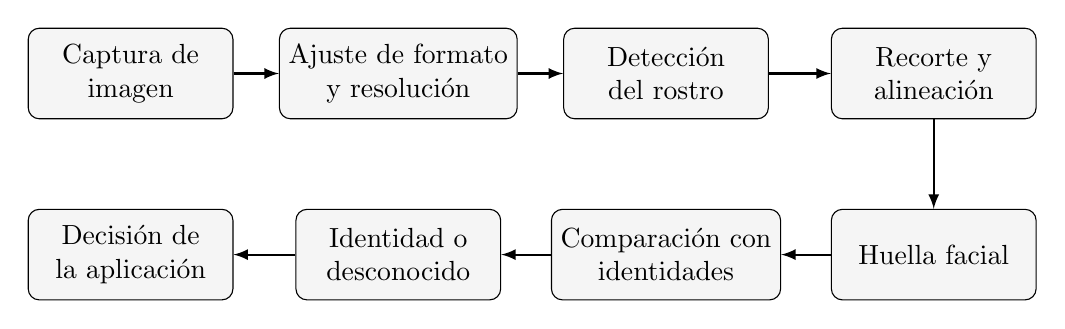
\begin{tikzpicture}[
        bloque/.style={draw, rounded corners, align=center, minimum width=2.6cm,
        minimum height=1.15cm, fill=gray!8},
        flecha/.style={thick, -latex}
    ]
        \node[bloque] (camara) at (0,0) {Captura de\\imagen};
        \node[bloque] (pre) at (3.4,0) {Ajuste de formato\\y resolución};
        \node[bloque] (det) at (6.8,0) {Detección\\del rostro};
        \node[bloque] (ali) at (10.2,0) {Recorte y\\alineación};
        \node[bloque] (vec) at (10.2,-2.3) {Huella facial};
        \node[bloque] (comp) at (6.8,-2.3) {Comparación con\\identidades};
        \node[bloque] (res) at (3.4,-2.3) {Identidad o\\desconocido};
        \node[bloque] (accion) at (0,-2.3) {Decisión de\\la aplicación};
        \draw[flecha] (camara) -- (pre);
        \draw[flecha] (pre) -- (det);
        \draw[flecha] (det) -- (ali);
        \draw[flecha] (ali) -- (vec);
        \draw[flecha] (vec) -- (comp);
        \draw[flecha] (comp) -- (res);
        \draw[flecha] (res) -- (accion);
    \end{tikzpicture}%
    }
    \caption{Flujo simplificado de un sistema de reconocimiento facial. Fuente: elaboración propia.}
    \label{fig:flujo_reconocimiento_facial}
\end{figure}

\subsection{Recursos computacionales del microcontrolador}

Para ejecutar aplicaciones de visión artificial, un microcontrolador debe
almacenar la imagen capturada y los datos temporales generados durante su
procesamiento. Entre los recursos utilizados se encuentran la memoria flash, la
RAM interna, la PSRAM y la capacidad de procesamiento de la CPU. Los modelos
también requieren memoria para sus entradas, resultados intermedios y salidas,
mientras que las imágenes de mayor resolución y el uso de varios búferes
aumentan el espacio necesario \cite{ESPDLModelExecution,ESP32Camera}. Los
recursos principales se resumen en la
Tabla~\ref{tab:recursos_vision_embebida}.

\begin{table}[H]
    \centering
    \caption{Recursos principales para la ejecución de visión artificial en un
    sistema embebido. Fuente: elaboración propia con base en
    \cite{TinyMLReview2022,ESPDLModelExecution,ESP32Camera}.}
    \label{tab:recursos_vision_embebida}
    \begin{tabularx}{\textwidth}{p{0.18\textwidth} X}
        \toprule
        \textbf{Recurso} & \textbf{Función dentro del sistema} \\
        \midrule
        Memoria flash & Almacena el programa, los parámetros de los modelos y
        datos que deben conservarse después de apagar el dispositivo. \\
        RAM interna & Mantiene variables, resultados temporales y estructuras
        utilizadas durante la ejecución. Es rápida, pero su capacidad es
        limitada. \\
        PSRAM & Memoria externa utilizada para contener imágenes, búferes de la
        cámara y otros datos que no caben en la RAM interna. Su contenido se
        pierde al retirar la alimentación. \\
        CPU & Ejecuta el programa y las operaciones matemáticas del algoritmo.
        Su velocidad determina, en parte, cuántas imágenes pueden analizarse por
        segundo. \\
        NPU & Unidad especializada disponible en algunos procesadores para
        acelerar redes neuronales. No todos los dispositivos de bajo costo
        incorporan este tipo de unidad. \\
        \bottomrule
    \end{tabularx}
\end{table}

En este proyecto se utilizarán microcontroladores de la familia ESP32. En
particular, las tareas de captura y reconocimiento facial serán ejecutadas por
un ESP32-S3, por lo que resulta necesario considerar los recursos disponibles
en este dispositivo.

El ESP32-S3 no incorpora una unidad de procesamiento neuronal (NPU) dedicada.
En su lugar, ejecuta las operaciones mediante sus núcleos de procesamiento e
incorpora instrucciones vectoriales que permiten acelerar cálculos utilizados
en procesamiento de señales y redes neuronales. El dispositivo también admite
memoria flash y PSRAM externa, recursos importantes debido al espacio requerido
por las imágenes y los datos temporales del procesamiento
\cite{ESP32S3Datasheet}.

Específicamente, el ESP32-S3 integra dos núcleos Xtensa LX7 de hasta 240~MHz y
512~KB de SRAM interna. La PSRAM puede utilizarse para almacenar cuadros y
búferes de la cámara, mientras que la RAM interna mantiene variables y datos
que requieren acceso rápido durante la inferencia. Por su parte, la memoria
flash conserva el programa y los parámetros del modelo aun cuando se retire la
alimentación \cite{ESP32S3Datasheet,ESPDLModelExecution,ESP32Camera}.

\begin{figure}[H]
    \centering
    \resizebox{0.94\textwidth}{!}{%
    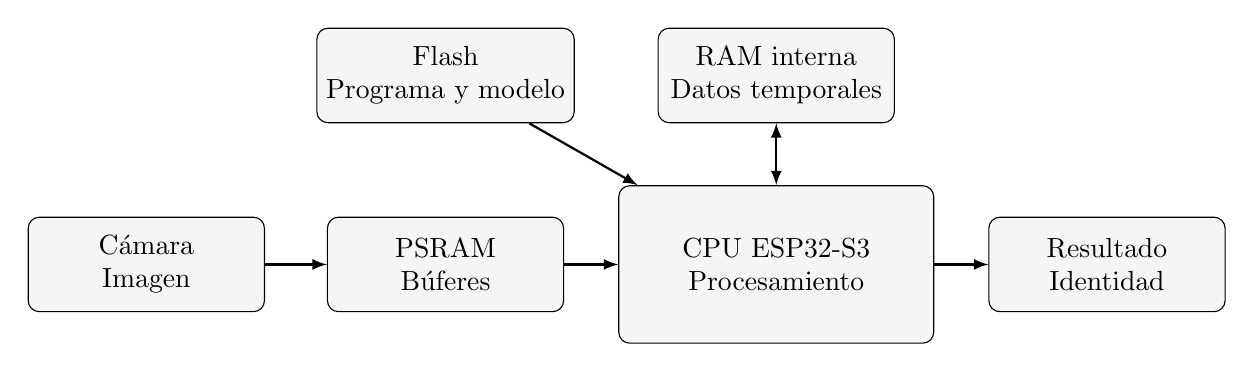
\begin{tikzpicture}[
        bloque/.style={draw, rounded corners, align=center, minimum width=3cm,
        minimum height=1.2cm, fill=gray!8},
        flecha/.style={thick, -latex}
    ]
        \node[bloque] (cam) at (0,0) {Cámara\\Imagen};
        \node[bloque] (psram) at (3.8,0) {PSRAM\\Búferes};
        \node[bloque, minimum width=4cm, minimum height=2cm] (cpu) at (8,0)
        {CPU ESP32-S3\\Procesamiento};
        \node[bloque] (ram) at (8,2.4) {RAM interna\\Datos temporales};
        \node[bloque] (flash) at (3.8,2.4) {Flash\\Programa y modelo};
        \node[bloque] (salida) at (12.2,0) {Resultado\\Identidad};
        \draw[flecha] (cam) -- (psram);
        \draw[flecha] (psram) -- (cpu);
        \draw[flecha] (flash) -- (cpu);
        \draw[latex-latex, thick] (ram) -- (cpu);
        \draw[flecha] (cpu) -- (salida);
    \end{tikzpicture}%
    }
    \caption{Uso simplificado de los recursos del ESP32-S3 durante una
    inferencia. Fuente: elaboración propia con base en
    \cite{ESP32S3Datasheet,ESPDLModelExecution,ESP32Camera}.}
    \label{fig:recursos_vision_esp32s3}
\end{figure}

\subsection{Estrategias para reducir los recursos necesarios}

La idea de un algoritmo ligero es sencilla: utilizar solo los datos y cálculos
necesarios para obtener un resultado útil. Una primera medida es trabajar con
una imagen más pequeña. Si la resolución disminuye, existen menos píxeles que
guardar y analizar, por lo que el procesamiento puede ser más rápido. Sin
embargo, no conviene reducirla demasiado, porque el rostro podría perder el
detalle necesario para distinguir a una persona
\cite{MobileNet2017,MCUNet2020}.

También puede evitarse el análisis completo de cada imagen. Primero se detecta
dónde está el rostro y después se procesa únicamente esa región
\cite{ESPWHOGetStarted2026}. De forma similar, una aplicación que no requiere
video fluido puede capturar y analizar imágenes a determinados intervalos. Esto
reduce la carga de procesamiento y permite liberar cada imagen antes de
capturar la siguiente.

Otra técnica es la cuantización. En lugar de representar los cálculos del modelo
con números grandes de punto flotante, se utilizan enteros más pequeños, por
ejemplo de 8 o 16 bits. Esto facilita que el modelo se almacene y ejecute en un
microcontrolador. ESP-DL utiliza modelos cuantizados en su formato
\texttt{.espdl} y ofrece herramientas para convertirlos y comprobar su exactitud
\cite{ESPDLQuantization}.

\subsection{Bibliotecas ESP-DL y ESP-WHO}

ESP-DL es una biblioteca desarrollada por Espressif para ejecutar modelos de
aprendizaje profundo en sus microcontroladores. Incluye operaciones matemáticas,
administración de memoria, carga de modelos y funciones optimizadas para las
instrucciones disponibles en cada dispositivo. Su finalidad es facilitar la
inferencia, es decir, la ejecución de un modelo previamente preparado para
obtener un resultado a partir de nuevos datos \cite{ESPDLGuide}.

ESP-WHO es una plataforma de visión artificial construida sobre ESP-DL. Incluye
ejemplos para detección y reconocimiento facial, detección de personas y otras
aplicaciones de visión. Estos ejemplos proporcionan una base que puede adaptarse
a una aplicación particular sin desarrollar desde cero todas las etapas de
captura y análisis de imágenes \cite{ESPWHO}.

\begin{figure}[H]
    \centering
    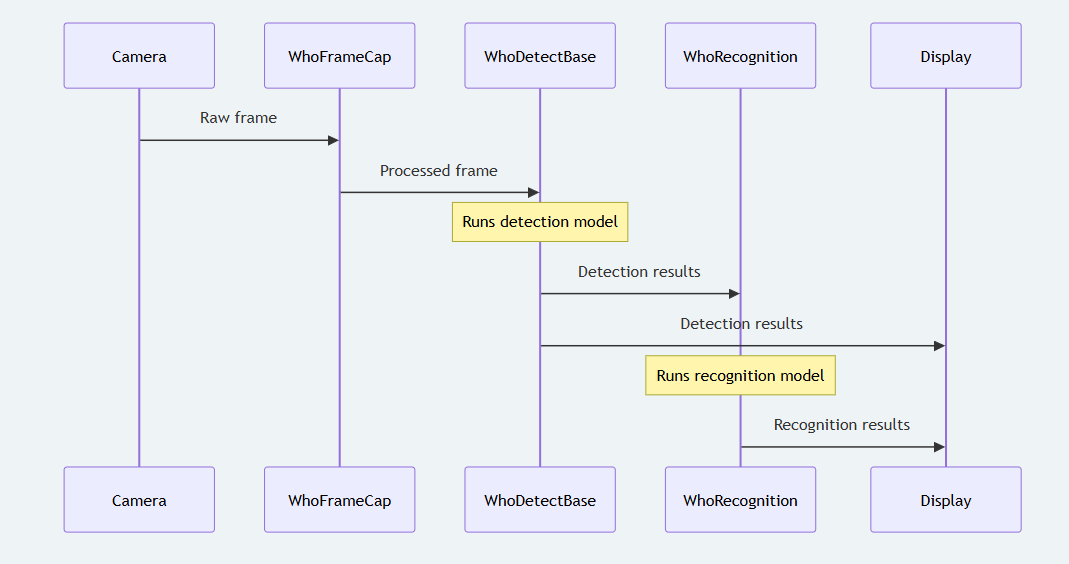
\includegraphics[width=\textwidth]{pics/TF_07.png}
    \caption{Diagrama de bloques de flujo de operación para reconocimiento facial 
    utilizando ESP-WHO \cite{ESPWHOGetStarted2026}.}
    \label{fig:modelo_espnow}
\end{figure}

La relación puede entenderse por niveles: \texttt{esp\_camera} adquiere la
imagen; ESP-DL ejecuta las operaciones del modelo; ESP-WHO organiza las etapas
de la aplicación; y el código del proyecto decide qué hacer con el resultado.
El entrenamiento del modelo se realiza normalmente en una computadora con
mayores recursos, mientras que el microcontrolador ejecuta la inferencia con
imágenes nuevas. Esta separación convierte a ESP-WHO en un punto de partida
apropiado para estudiar una solución de bajo costo.

Por otra parte, el componente \texttt{esp\_camera} se encarga de configurar la
cámara y obtener sus imágenes. En proyectos desarrollados con el núcleo de
Arduino para ESP32, este controlador ya se encuentra integrado. La documentación
recomienda utilizar PSRAM cuando se requieren varios búferes o resoluciones
mayores \cite{ESP32Camera,ArduinoCameraWebServer}. Por tanto,
\texttt{esp\_camera} realiza la adquisición de la imagen, mientras que ESP-DL y
los componentes asociados realizan su análisis.

% Picture here about the relationship between esp_camera, ESP-DL, ESP-WHO and
% the application developed by the user.

\subsection{Limitaciones generales del reconocimiento facial embebido}

El reconocimiento facial depende mucho de la imagen que recibe. Un rostro
frontal, enfocado y con iluminación uniforme ofrece mejores condiciones. En
cambio, el contraluz, el movimiento, una distancia inadecuada, un rostro de
perfil o una mascarilla pueden ocultar información importante. NIST incluye
factores como enfoque, iluminación, ruido, posición de la cabeza y expresión
facial dentro de la evaluación de calidad de una imagen
\cite{NISTFaceImageQuality,Shepley2019FaceRecognition}.

Incluso con una imagen adecuada pueden existir errores. Una
\textit{falsa aceptación} ocurre cuando el sistema confunde a una persona con
otra; un \textit{falso rechazo} ocurre cuando no reconoce a alguien que sí estaba
registrado. El umbral de comparación influye en ambos errores: hacerlo más
estricto puede reducir las aceptaciones incorrectas, pero también puede aumentar
los rechazos \cite{NISTFRVT}.

Además, reconocer un rostro no confirma por sí solo que hay una persona real
frente a la cámara. Una fotografía o un video podrían requerir controles
adicionales conocidos como detección de vida (\textit{liveness detection}).
Tampoco es razonable esperar el mismo desempeño de una computadora y de un
microcontrolador: utilizar más resolución o un modelo más grande puede mejorar
el análisis, pero consume más memoria y tarda más. Por esta razón, la exactitud
debe indicarse junto con las condiciones de captura y el equipo utilizado, no
como un porcentaje que siempre será igual \cite{ESPDLPerformance}.
